\part{Capitulo 4}
\vspace{-0.3cm}
\begin{center}
    \begin{large}
        Metodos Probabilisticos y Estadisticos
    \end{large}
\end{center}

La mayor parte de los procesos hidrologicos son aleatorios, no existen procesos puramente deterministicos. En consecuencia, para poder hacer una caracterizacion se \textbf{debe registrar la ocurrencia de ellos} mediante registros historicos, los cuales son sometidos a un post procesado estadistico.
\\ \\
Los objetivos son los siguientes:

\begin{itemize}
    \item Estimacion de P( ) de que ocurra un determinado evento
    \item Estimacion de eventos que no han ocurrido o no se han observado
    \item Caracterizacion estadistica de series hidrologicas
    \item Correlacion y regrecion para completar y extender series
\end{itemize}

\section{Frecuencia Relativa y Acumulada}

La sumatoria de todas las frecuencias relativas debe ser igual a 1, es decir:

\begin{equation}
    \sum_{i=1}^{n} f_i = 1
\end{equation}

Estas funciones son obtenidas a partir de una muestra, por lo que se pueden obtener de estimaciones de la poblacion aproximando como limites:

\begin{figure}[H]
    \centering
    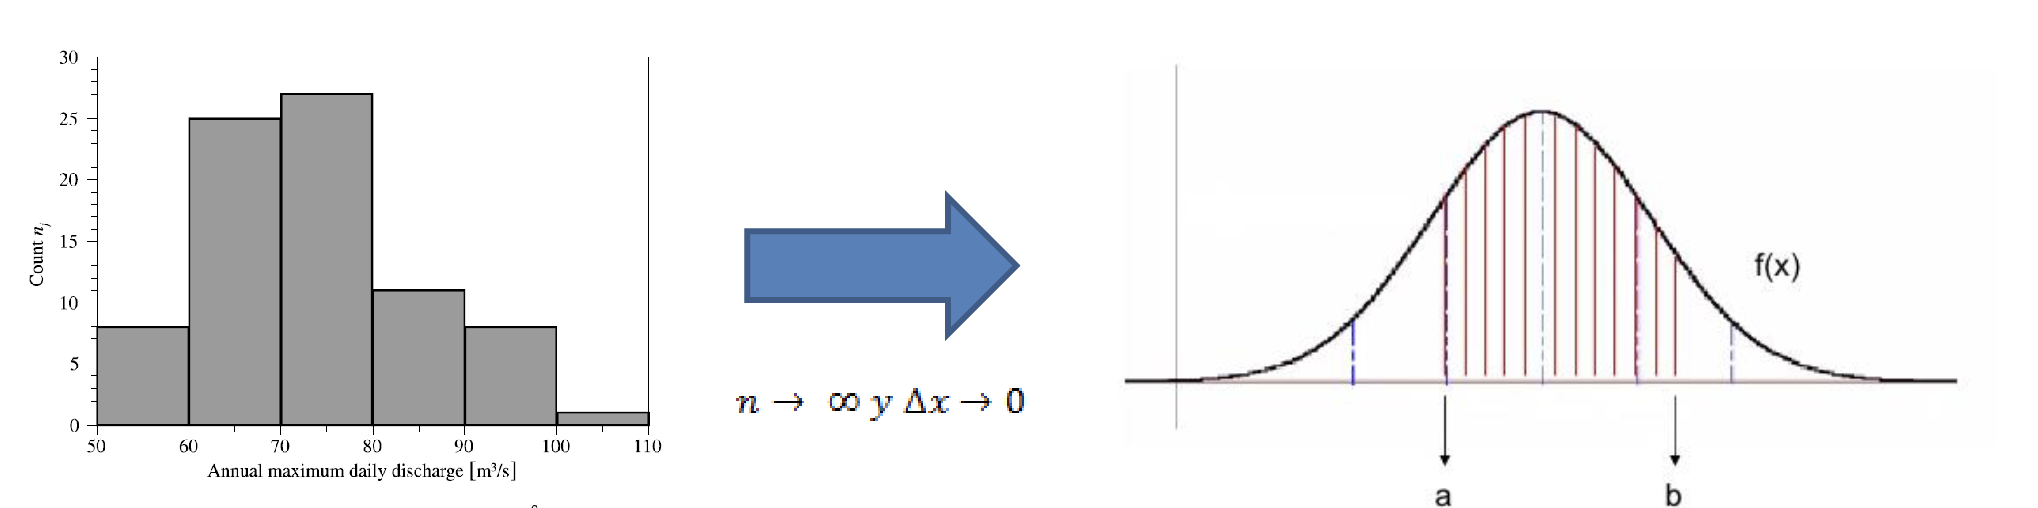
\includegraphics[width=0.85\textwidth]{imagenes/frecuencia.png}
    \label{fig:frecuencia_acumulada}
\end{figure}

\section{Periodo de Retorno y P( ) de Excedencia}

Se puede definir como: el intervalo de recurrencia promedio entre evnetos que igualan o excedan una magnitud especifica
\\ \\
Es decir, en un horizonte de tiempo grande, se esperaria observar eventos iguales o mayores cada \textbf{T años}.
\\ \\
Sea \textbf{p} la probabilidad de exito y \textbf{(1-p)} la probabilidad de falla en un determinado año. Podemos definir la \textbf{probabilidad de recurrencia $\pi$} como el producto de \textbf{$\pi$ - 1} fallas seguidas por un exito, por lo tanto:

\begin{equation}
    P(X > X_t) = \frac{1}{T}
\end{equation}

Ejemplo:

\begin{figure}[H]
    \centering
    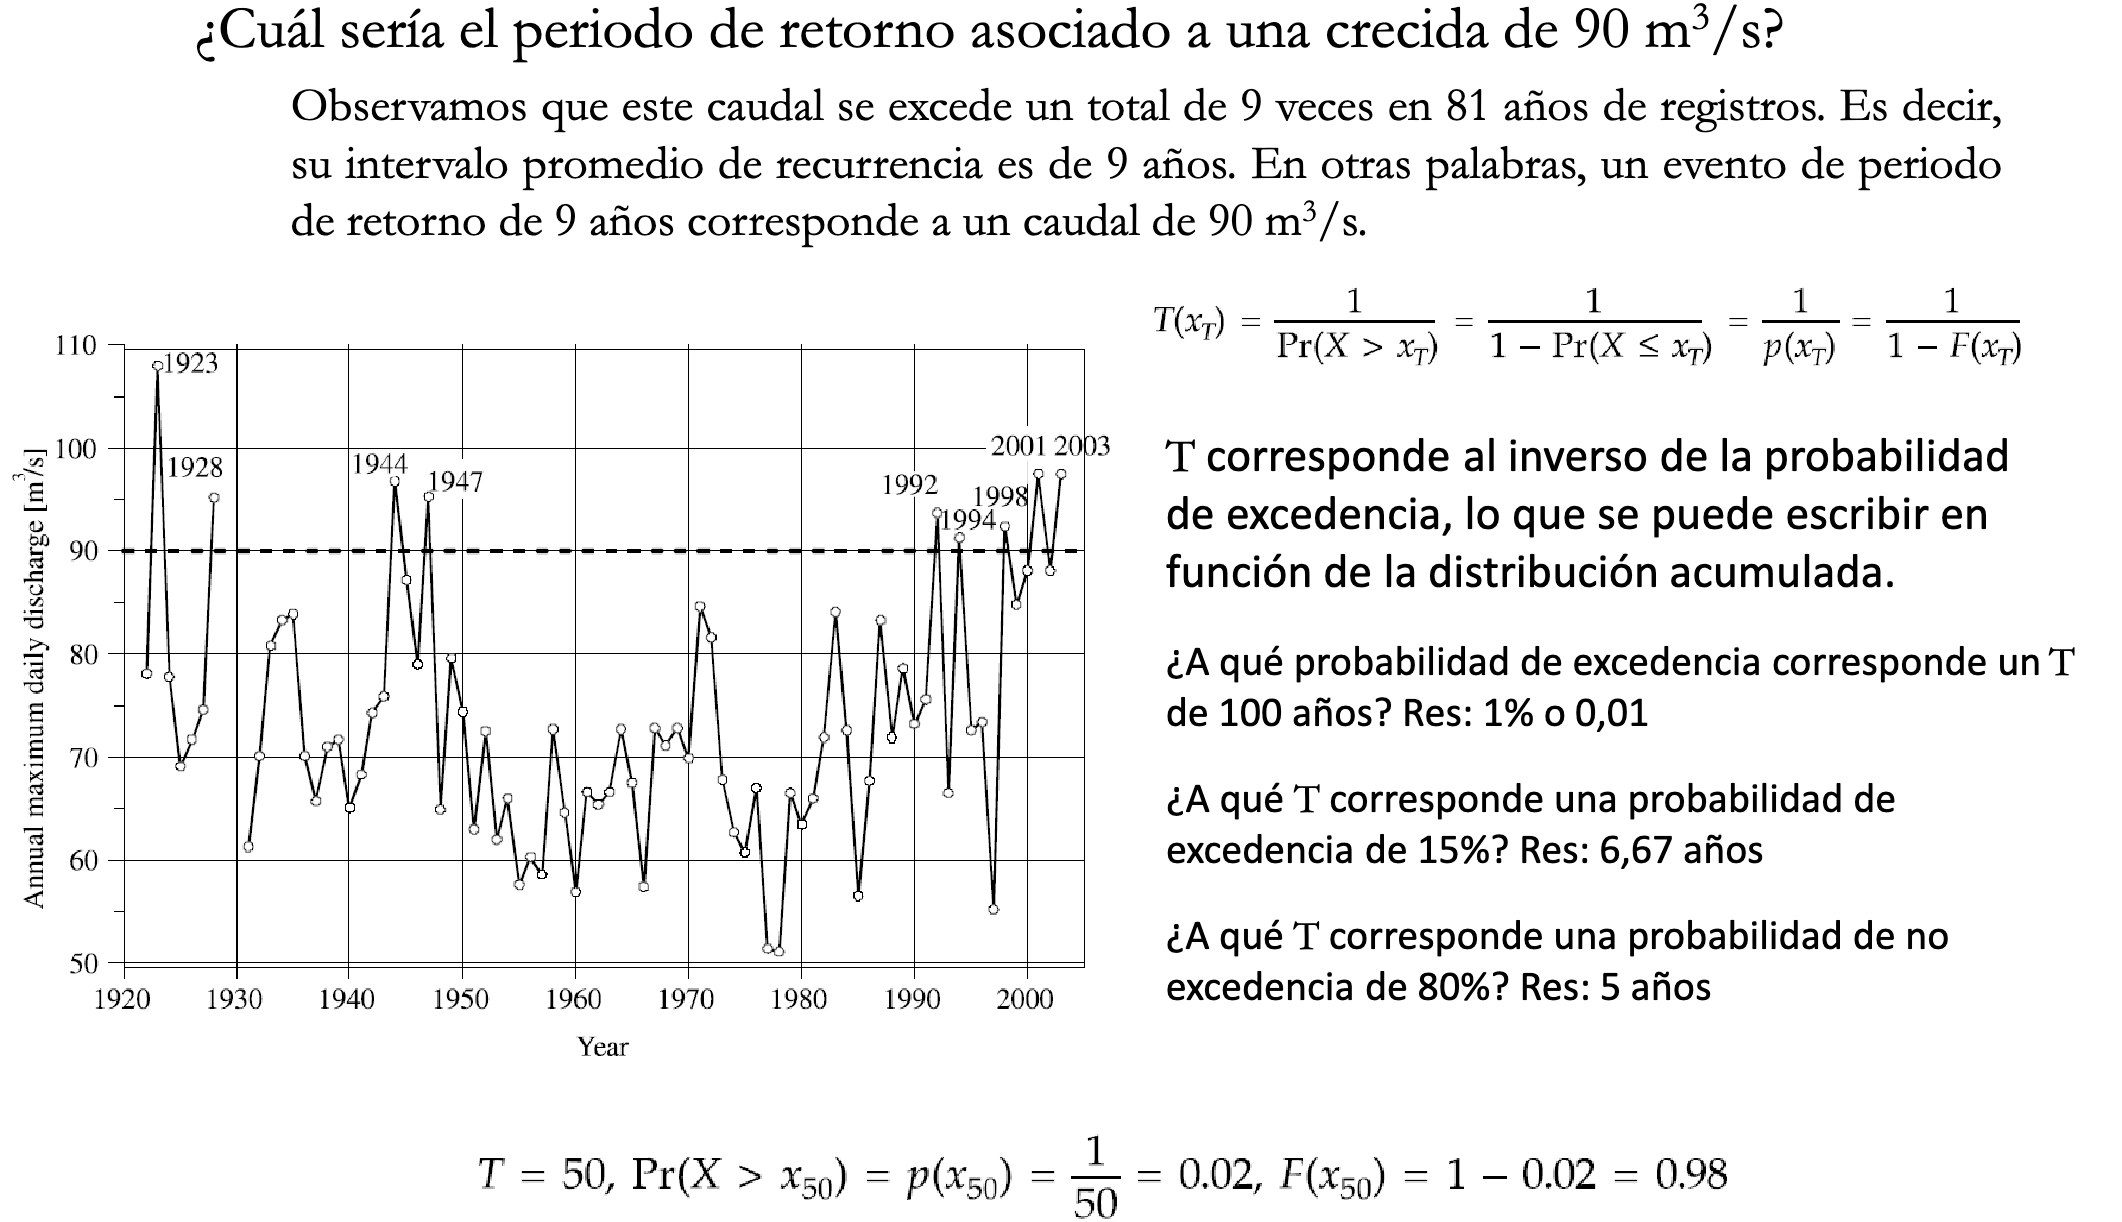
\includegraphics[width=0.85\textwidth]{imagenes/retorno.png}
    \label{fig:periodo_retorno}
\end{figure}

\section{Seguridad y Riesgo Hidrololgico}

Se define como la probabilidad de no excedencia:

\begin{equation}
    P_{no-exc} = 1 - \frac{1}{T}
\end{equation}

Por lo tanto, la probabilidad de que cierto valor no se exceda en n años es:

\begin{equation}
    S = (1 - \frac{1}{T})^n 
\end{equation}

Lo cual se define como \textbf{Seguridad Hidrologica}, donde su complemento es el \textbf{Riesgo Hidrologico}, lo cual se usa para obras hidraulicas:

\begin{equation}
    R = 1- S = 1 - (1 - \frac{1}{T})^n
\end{equation}

\textbf{Nota: aproximar el valor de t a un valor multiplo de 5}

\begin{figure}[H]
    \centering
    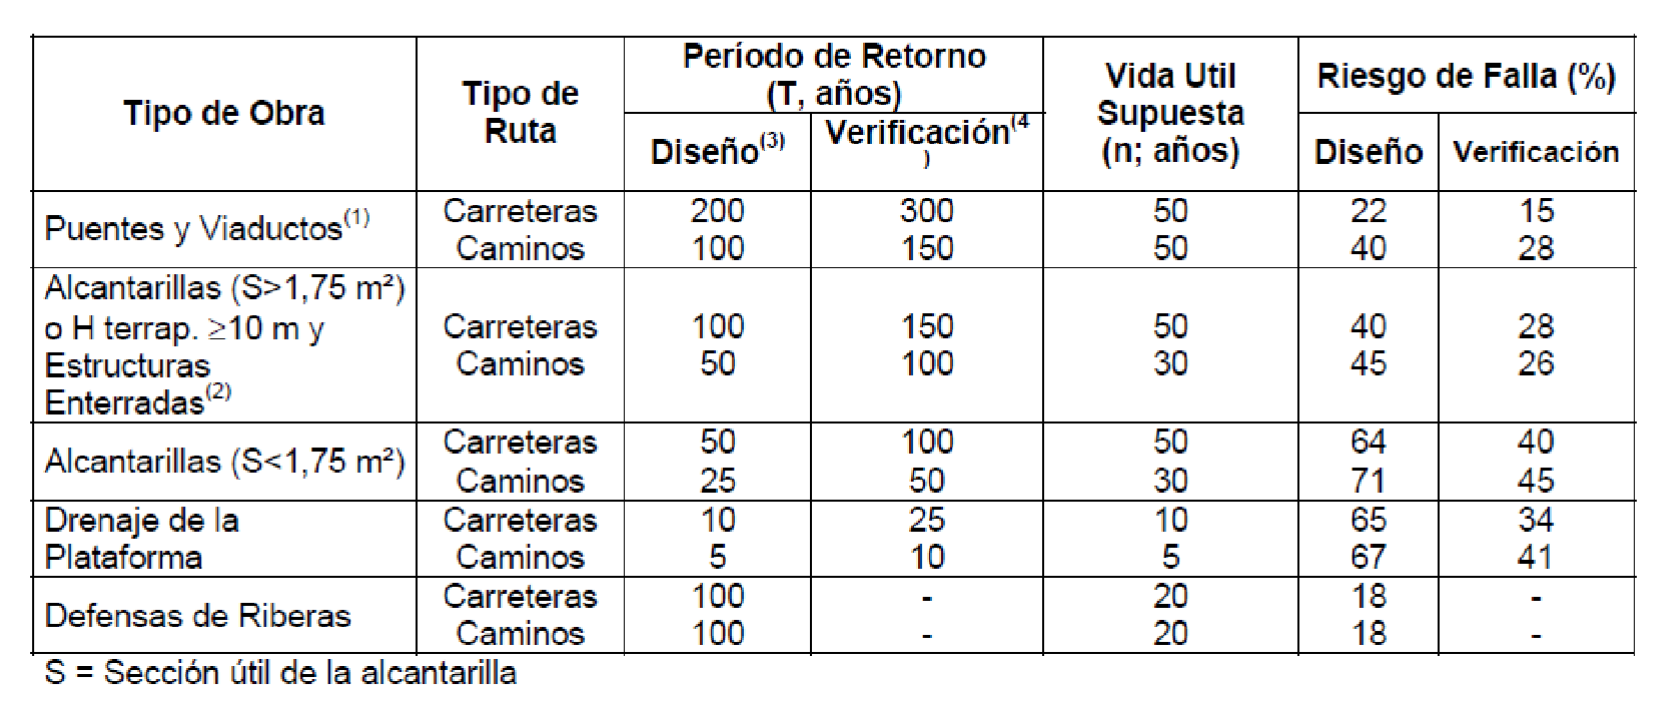
\includegraphics[width=0.85\textwidth]{imagenes/Qmi.png}
    \label{fig:Qmi}
\end{figure}

\section{Distribuciones Discretas}

\subsection{Bernoulli}

Una variable aleatoria posee dos estados, exito o fracaso, por lo tanto puede ser 1 o 0. Por lo tanto:

\begin{equation}
    P(X = 1) = p
\end{equation}

\begin{equation}
    P(X = 0) = 1 - p
\end{equation}

\subsection{Distribucion Binomial}

Este modelo surge a partir de la realizacion de n ensayos independientes tipo bernoulli, donde se define una variable aleatorioa k como el numero de exitos que ocurren en n ensayos, por lo tanto:

\begin{equation}
    P(X = k) = \binom{n}{k} \cdot p^k \cdot (1-p)^{n-k}
\end{equation}

Donde:

\begin{equation}
    \binom{n}{k} = \frac{n!}{k!(n-k)!}
\end{equation}

Y K es el numero de evnetos exitosos.
\\ \\
Cada evento climatologico es independiente, por lo tanto es un ensayo tipo bernoulli, y su conjunto se representa binomialmente

\section{Parametros Estadisticos}

\subsection{Varianza}

Se denomina a la varianza \textbf{$s^2$} como la media de los cuadrados de las diferencias entre cada valor y la media, por lo tanto:
\\ \\
Caso discreto: 

\begin{equation}
    s^2 = \frac{\sum_{i=1}^{n} (x_i - \bar{x})^2}{n-1}
\end{equation}

Caso continuo:

\begin{equation}
    \sigma^2 = E((x-\mu)^2)
\end{equation}

\subsection{Desviacion Estandar}

Se define como la raiz cuadrada de la varianza, por lo tanto:

\begin{equation}
    s = \sqrt{s^2}
\end{equation}

\subsection{Coeficiente de Variacion}

Se define como la relacion entre la desviacion estandar y la media, por lo tanto:

\begin{equation}
    CV = \frac{s}{\bar{x}}
\end{equation}

\subsection{Coeficiente de Asimetria}

Se define como la medida de asimetria de una distribucion, por lo tanto:

\begin{equation}
    \gamma = \frac{E((x-\mu)^3)}{\sigma^3}
\end{equation}

\section{Distribuciones Continuas}

\subsection{Distribucion Normal}

Se define como:

\begin{equation}
    f(x) = \frac{1}{\sigma\sqrt{2\pi}} \cdot e^{-\frac{(x-\mu)^2}{2\sigma^2}}
\end{equation}

Donde $\mu$ es la media y $\sigma$ la desviacion estandar.
\\ \\
Esta funcion no es integrable, por lo tanto para evaluar la funcion se utilizan tablas y o formulas aproximadas.
\\ \\
\textbf{El proceso de normalizacion consiste en reemplazar la variable original por una nueva variable estandarizada (z) }

\begin{equation}
    z = \frac{x-\mu}{\sigma}
\end{equation}

De esta forma se obtiene:

\begin{equation}
    f(x) = \frac{1}{\sqrt{2\pi}} \cdot e^{-\frac{z^2}{2}}
\end{equation}

\subsection{Distribucion Log Normal}

Es una transformacion de la distribucion Normal, donde se modela de una forma asimetrica con respecto a un valor medio, por ejemplo para precipitaciones o caudales:

\begin{equation}
    f(x) = \frac{1}{\sigma_y\sqrt{2\pi}} \cdot e^{\frac{1}{2}(\frac{y-\mu_y}{\sigma_y})^2}
\end{equation}

Donde los parametros se estiman en base a la muestra aplicando log a las variables observadas:

\begin{equation}
    \mu_y = \bar{y} = \frac{1}{N} \sum_{i=1}^{N} \ln(x_i)
\end{equation}

\subsection{Distribución de Valores Extremos}

Los datos en hidrología suelen ser series de valores extremos o excedencias anuales (máximos o mínimos).

Distribución de Valor Extremo General (DVEG):

\begin{equation}
    F(x) = \exp \left\{ - \left[ 1 - \kappa \left( \frac{x - u}{\alpha} \right) \right]^{1/\kappa} \right\}
\end{equation}

Existen 3 tipos de distribuciones extremas:

\begin{enumerate}
    \item Gumbel: $\kappa = 0$ en DVEG
    \begin{equation}
        F(x) = \exp\left[-\exp\left(-\frac{x-u}{\alpha}\right)\right]
    \end{equation}
        
    \begin{equation}
        \alpha = \frac{\sqrt{6} \cdot \sigma}{\pi}
        \quad \text{y} \quad
        u = \bar{x} - 0.5722 \cdot \alpha
    \end{equation}

    Variable reducida:

    \begin{equation}
        y = \frac{x-u}{\alpha}
    \end{equation}

    Finalmente:

    \begin{equation}
        y_T = -\ln(-\ln\left(\frac{T-1}{T}\right))
    \end{equation}

    \begin{equation}
        x_T = u + \alpha \cdot Y_T
        \quad \text{;} \quad
        Y_T \rightarrow y = \frac{x-u}{\alpha} 
    \end{equation}

    Esta expresión permite calcular el valor asociado a un evento de periodo de retorno T, en función del promedio, desv. estándar y T.
    \\\\
    Si la muestra es de tamaño finito, se debe corregir el valor de $\alpha$ y $u$:

    \begin{equation}
        \alpha = \frac{\sigma_x}{\sigma_n}
    \end{equation}

    \begin{equation}
        u = \bar{x} - \sigma_x \cdot \frac{y_n}{\sigma_n}
    \end{equation}

    Los valores de $\sigma_n$ y $y_n$ se obtienen de tablas.

    \item Fretcher: $\kappa < 0$
    \item Weibull: $\kappa > 0$
\end{enumerate}

\subsection{Distribución Pearson III}

\begin{equation}
    f(x) = \frac{1}{\alpha \cdot \Gamma(\beta)} \left[\frac{x - \gamma}{\alpha}\right]^{\beta - 1} \cdot \exp\left[-\frac{x - \gamma}{\alpha}\right]
\end{equation}
    
\begin{equation}
    \alpha = \frac{\sigma}{\sqrt{\beta}}
\end{equation}
    
\begin{equation}
    \beta = \left(\frac{2}{C_s}\right)^2
\end{equation}
    
\begin{equation}
    \gamma = \mu - \sigma \cdot \sqrt{\beta}
\end{equation}
    
\section{Análisis de Frecuencia}

\subsection{Periodo de Retorno (T)}

Cálculo o estimación de eventos extremos requiere que la función de pbb F(x) sea invertible. El análisis de frecuencia ayuda a determinar un x sin una función invertible.
\\\\
Periodo de retorno de un evento(T): Intervalo de recurrencia promedio entre eventos que igualan o exceden una magnitud especificada.

\begin{equation}
    P = 1/T
\end{equation}

Donde P es la pbb de ocurrencia del evento.
\\\\

Los datos deben discretizarse para su análisis, donde con el total se pueden formar:
\begin{itemize}
    \item Series de duración completa
    \item Series de duración parcial
    \item Series de valores extremos
    \item Series de excedencias: Se define umbral de la variable analizada para obtener una serie con los N mayores valores.
    \item Serie de máximos: Se selecciona el máximo valor de cada año.
\end{itemize}

El objetivo del análisis de frecuencia es definir la distribución de mejor ajuste.
\\\\
Si se tienen registros fluviométricos, se puede construir la serie de caudales máximos.
\begin{equation}
    X_T = \mu + K_T \cdot \sigma
\end{equation}

Donde:
\begin{itemize}
    \item $X_T$: Valor asociado al periodo de retorno T
    \item $\mu$: Media de la serie
    \item $\sigma$: Desviación estándar de la serie
    \item $K_T$: Coeficiente de frecuencia (depende de distribución seleccionada y T) 
\end{itemize}

\subsubsection{Método del factor de frecuencia (Kt)}

\begin{figure}[H]
    \centering
    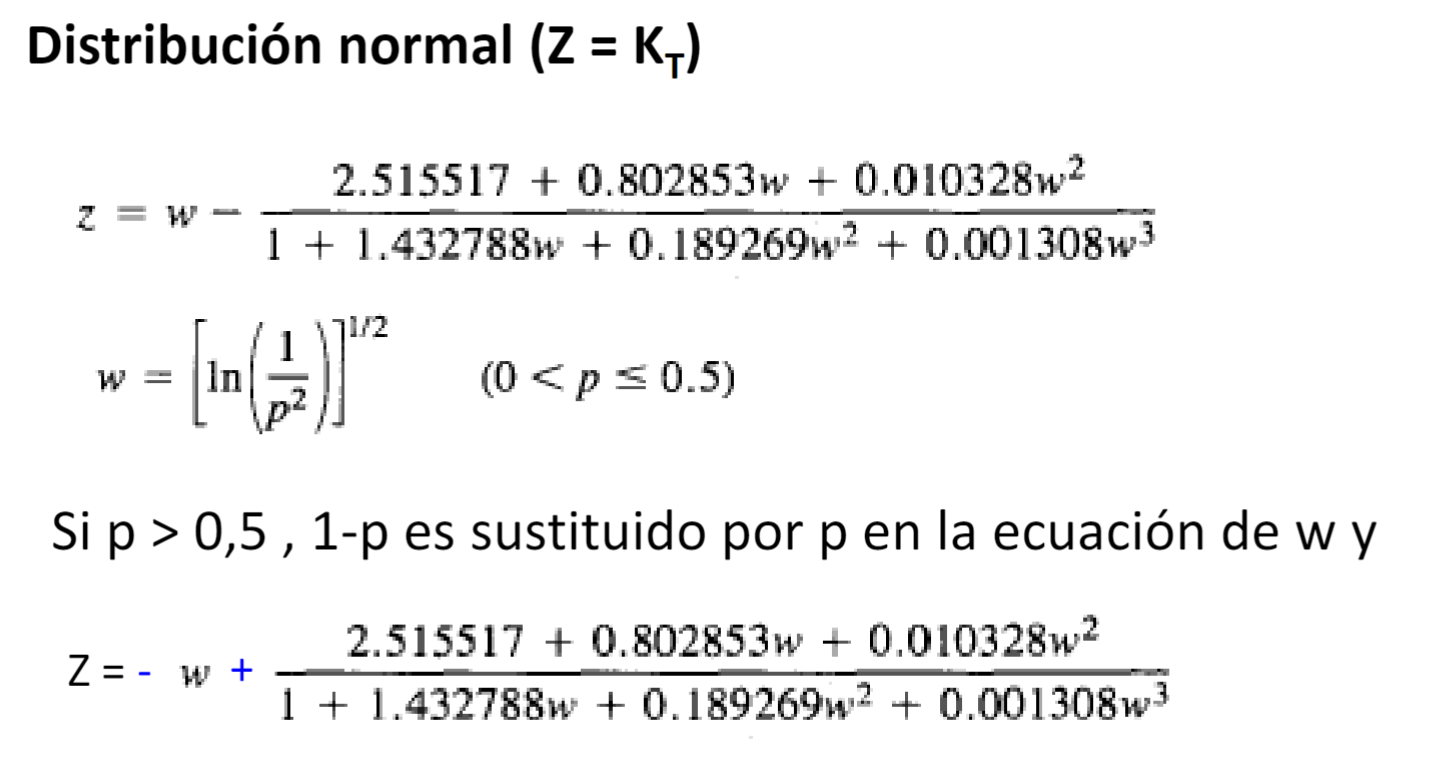
\includegraphics[width=0.85\textwidth]{imagenes/kt_norm.png}
    \label{fig:kt_norm}
\end{figure}

Para el caso de log normal, es válido el mismo $K_T$ pero se ajusta a la serie $\log{(x)}$ y $\ln{(x)}$

\begin{figure}[H]
    \centering
    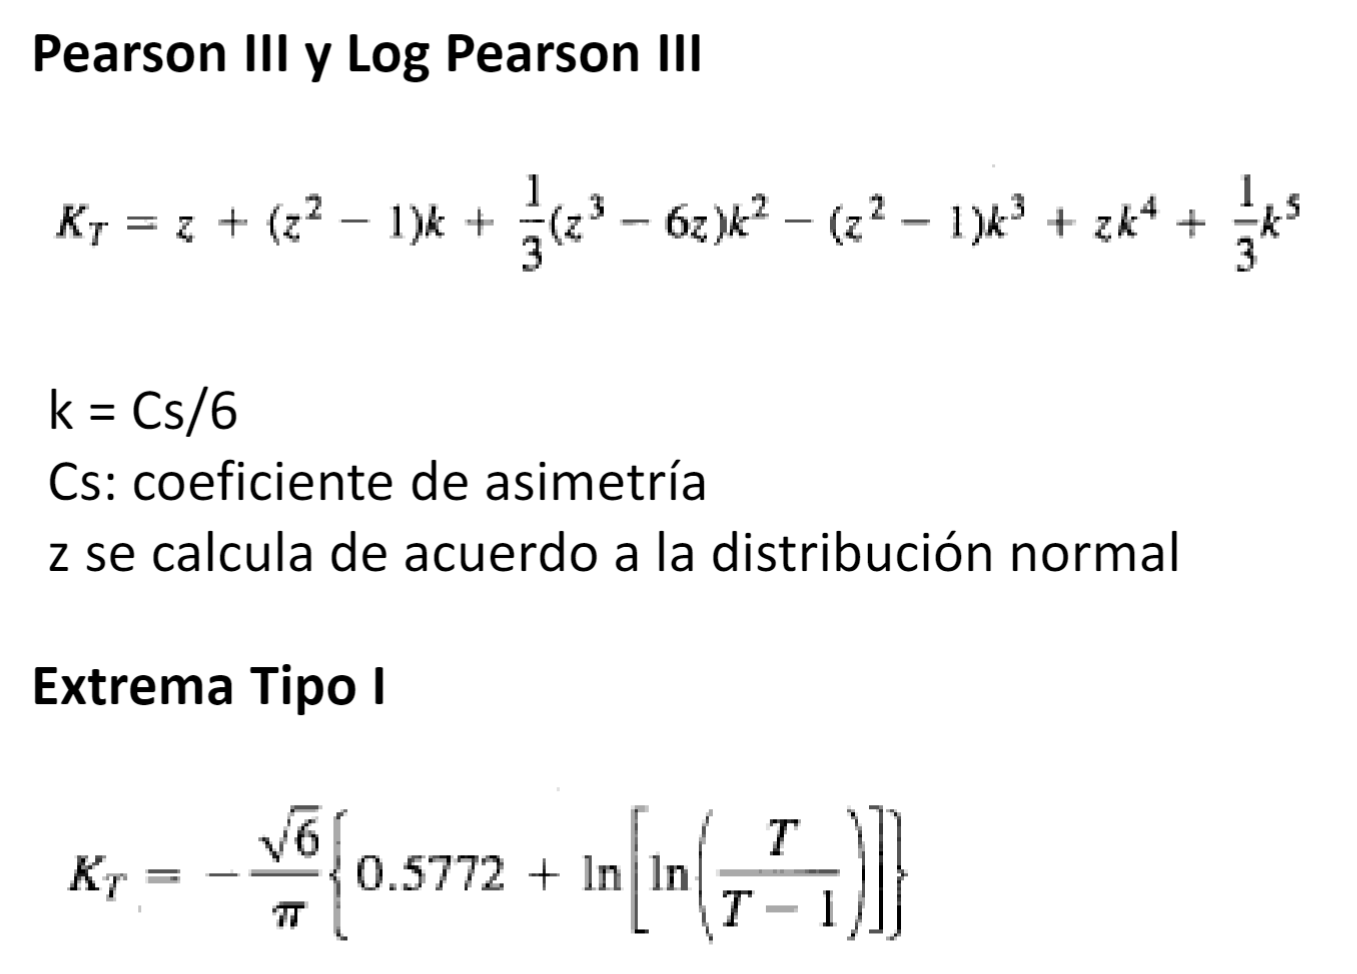
\includegraphics[width=0.85\textwidth]{imagenes/kt_2.png}
    \label{fig:kt_2}
\end{figure}

\begin{figure}[H]
    \centering
    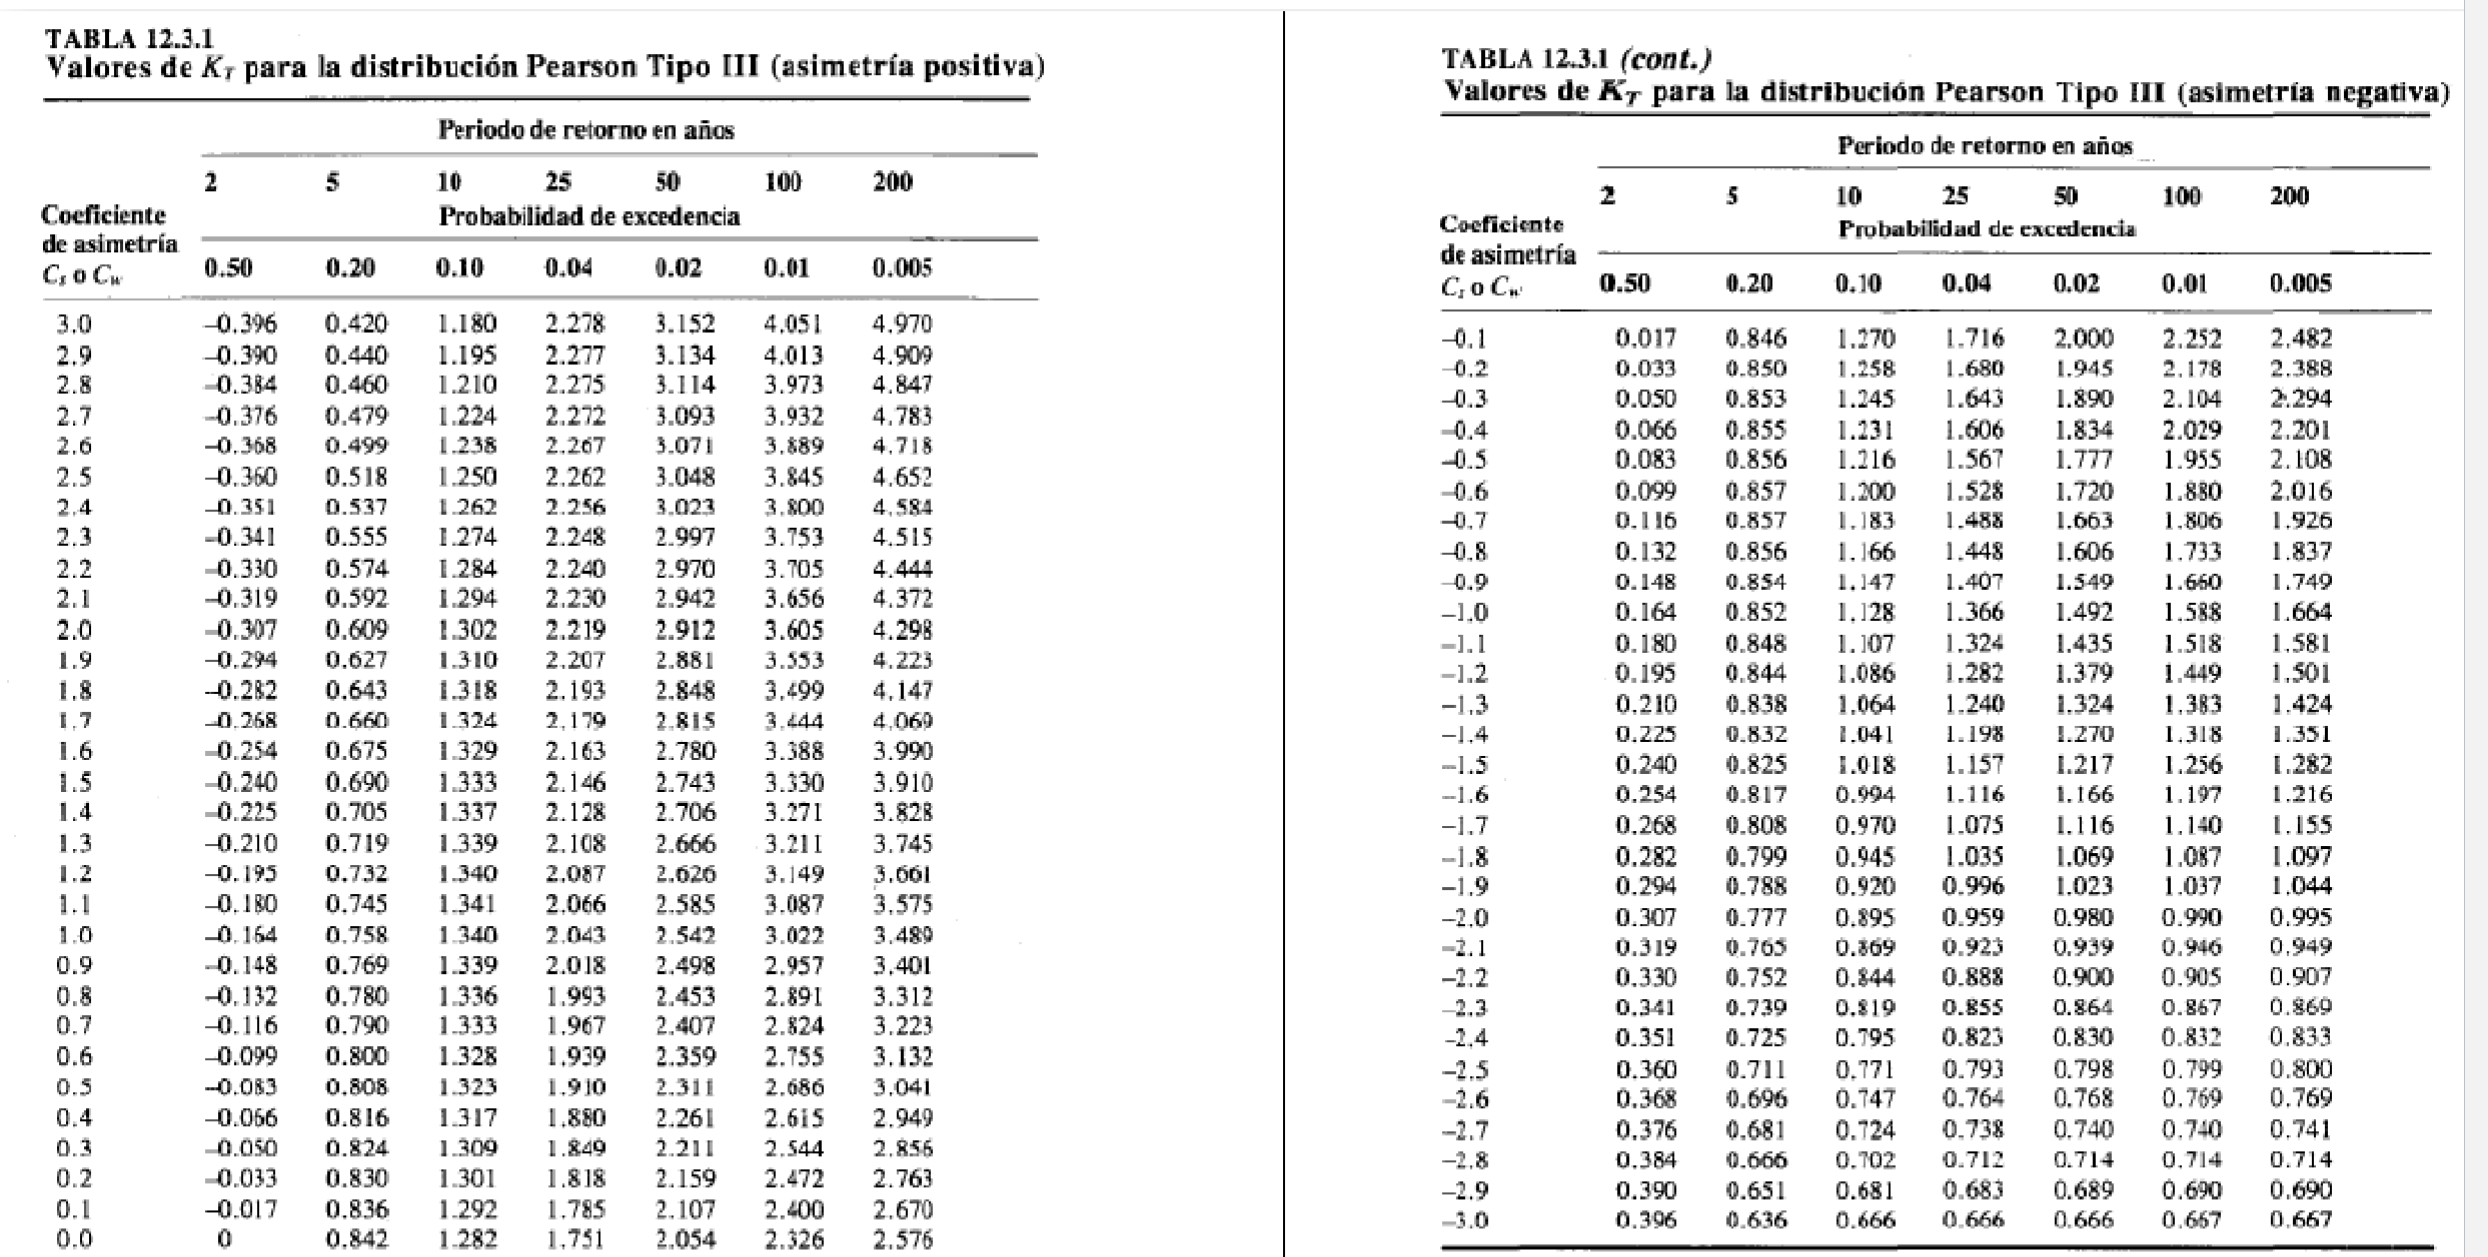
\includegraphics[width=1.1\textwidth]{imagenes/lista_kt.png}
    \label{fig:kt_3}
\end{figure}

Distribución Gumbel:

\begin{equation}
    K_T = \frac{Y_T-Y_n}{\sigma_n}
\end{equation}

\begin{equation}
    Y_T = -\ln\left(-\ln\left(\frac{T-1}{T}\right)\right)
\end{equation}

\subsubsection{Selección de la distribución que mejor ajusta}

\begin{enumerate}
    \item Métodos empíricos: Gráficos
    \item Métodos estadísticos: Test Chi-Cuadrado
\end{enumerate}

Se debe elegir la función de densidad de frecuencia que mejor represente la forma del histograma normalizado de la muestra.
\\\\
Método de Weibull:

\begin{enumerate}
    \item Se tienen datos estimados
    \item Se ordenam las observaciones en orden creciente o decreciente.
    \item A las observaciones se les asigna una probabilidad acumulada.
    \begin{equation}
        P(x>X) = \frac{m}{n+1} \text{, Para datos ordenados de mayor a menor}
    \end{equation}
    \item Graficar valores obtenidos Q vs Kt $\rightarrow$ Xt es caudal.
    \item Si los puntos siguen tendencia lineal, se acepta modelo.
\end{enumerate}

Error estandar:

\begin{figure}[H]
    \centering
    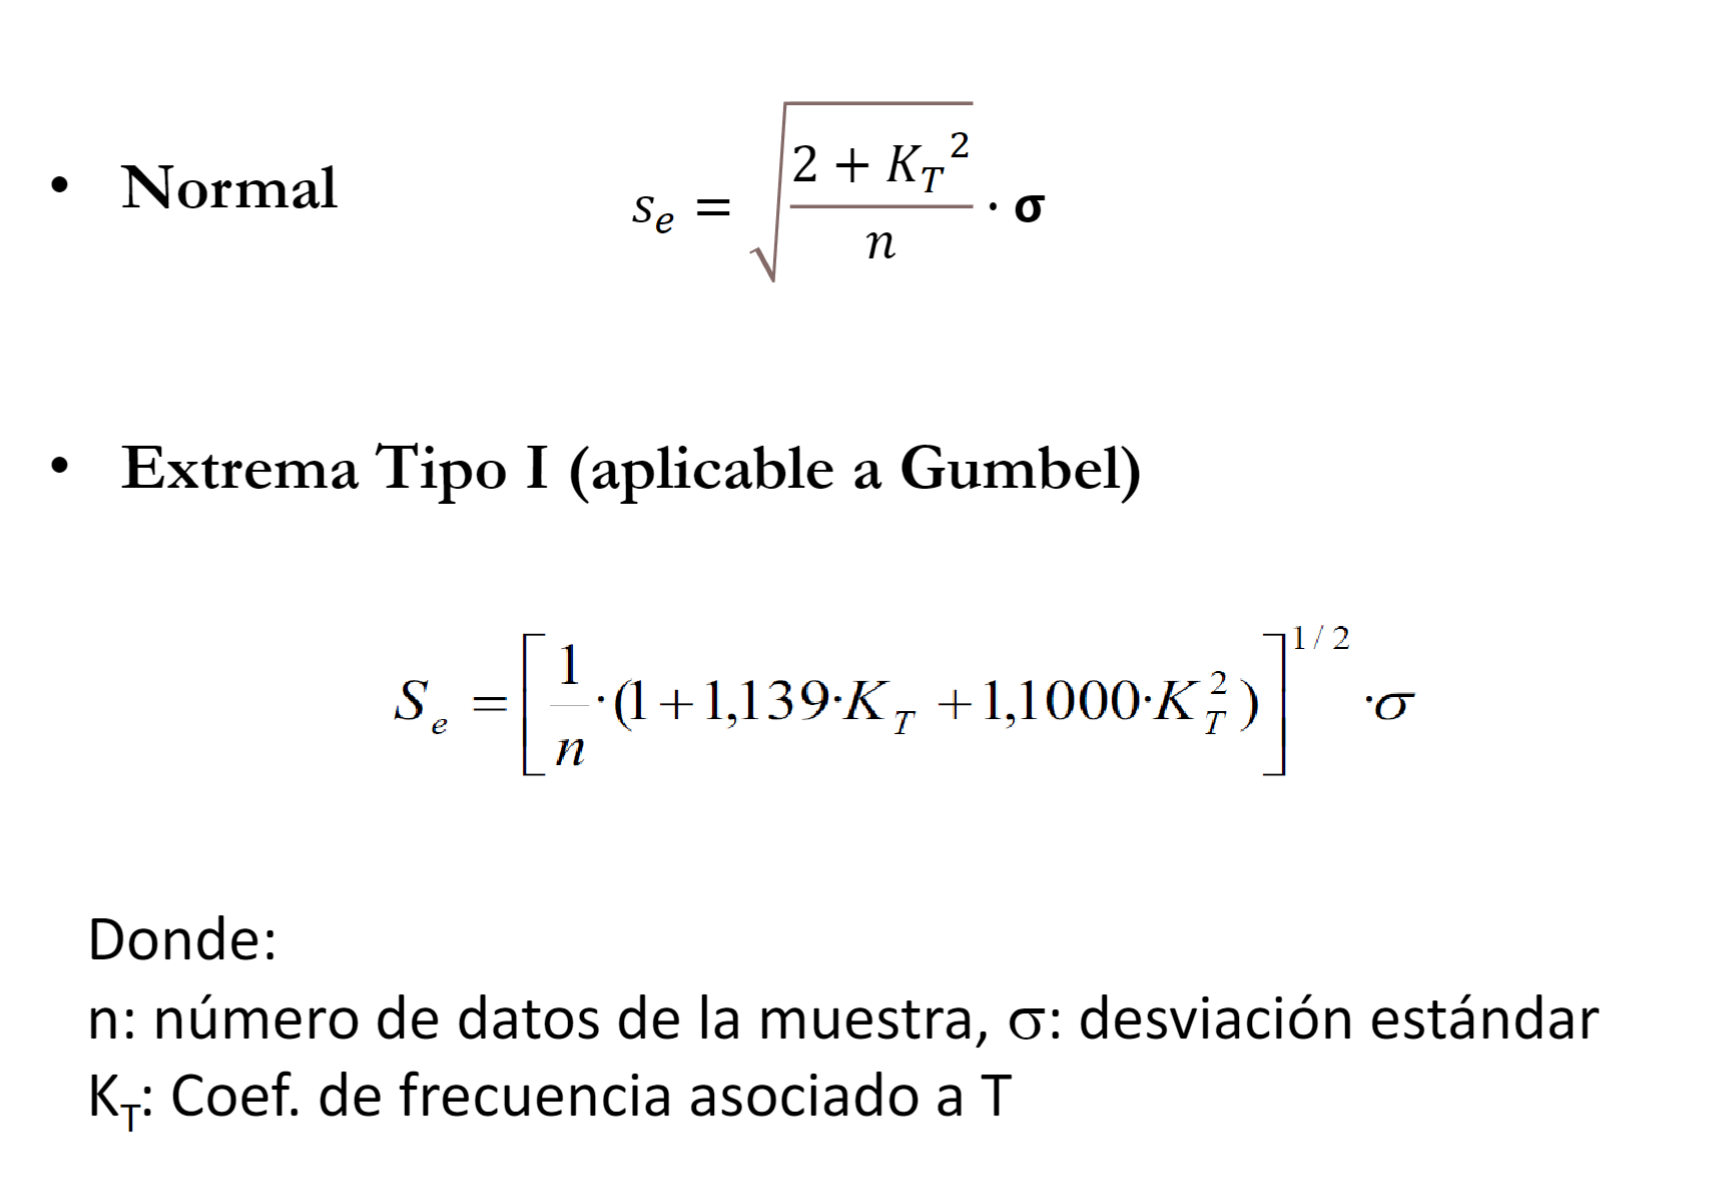
\includegraphics[width=0.85\textwidth]{imagenes/error_estandar.png}
    \label{fig:error_estandar}
\end{figure}

También estan los siguientes métodos:

\begin{itemize}
    \item Chi-Cuadrado
    \item Límites de confianza
\end{itemize}

¿Es correcto realizar un análisis de frecuencia a cualquier tipo de serie?

\begin{itemize}
    \item Las series de tiempo deben ser estacionarias. Estas son afectadas por:
    \begin{itemize}
        \item Factores climáticos
        \item Modificaciones a infraestructura
        \item Cambios en respuesta hidrológica de las cuencas
    \end{itemize}
    Se determina si es estacionaria con:
    \begin{itemize}
        \item Test de Mann-Kendall
        \item Test de Pettitt
    \end{itemize}

    \item Cambio climático $\rightarrow$ Serie no estacionaria.
    \begin{itemize}
        \item Se puede remover la tendencia a la serie, realizar AF y luego incorporar la tendencia.
        \item Se puede considerar serie cuasi-estacionaria de 30 años.
    \end{itemize}

    \item Si hacen falta datos se puede:
    \begin{itemize}
        \item Interpolar
        \item Regresión lineal
        \item Análisis de sequías o crecidas 
    \end{itemize}
\end{itemize}

